\chapter{Evaluation}

\section{Introduction}
CEP engines are used in a variety of scenarios, each of which has different requirements and settings, and that makes performance evaluation a true challenge. In fact there is not a universally agreed methodology of measurement and there are neither a reference workload, recorded from a real execution, nor a standard emulator, to generate a synthetic one.\\
So the first step, toward a better understanding of the strengths and limits of the system, was to define a base configuration and to create a tunable executor. Then we ran a reasonably wide range of tests exploring one by one the domains of the most relevant variables.\\
In this chapter I will analyze the results of a selected number of test cases, explaining why each configuration was chosen and how it could impact on a real world application.

\section{Environment}
\begin{table}[h]
  \begin{center}
    \begin{tabular}{|c|c|}
      \hline
      Processor: 		& Intel Core i7-4770 @ 3.40GHz\\
                        & 4 Cores, 8 Threads\\ 
      \hline
      RAM size: 		& 16GB\\
      \hline
      Operating System: & Debian GNU/Linux 8.6 (jessie)\\
                        & Kernel 3.16.0-4-amd64\\
      \hline
      C++ Compiler:     & G++ 4.9.2\\
      \hline
      Rust Compiler:    & 1.14.0-nightly (2016-11-05)\\
      \hline
    \end{tabular}
    \caption{Execution environment}
  \end{center}
\end{table}

\section{General Performances}
The complexity of creating an artificial workload is due to the vast combination of parameters that, interacting and influencing each other, characterize the execution of the application.\\
In a real world scenario most of those variables are bound to the environment and very specific: the inputs are correlated one each other and together deliver a meaningful information, at the same time the rules are manually tailored to the particular task.\\
On the opposite side, during a general purpose evaluation, it is necessary to control the behavior of the inputs and the complexity of the rules and it has to be done automatically, while preserving the stability of the execution. So the challenge is to create a model that is simple enough to predictably work under all the circumstances examined and rich enough to be interesting and customizable.

\subsection{Characteristic variables}
To find such a model we started analyzing the work done to test the TRex engine during the previous development phases.\\
Setting temporarily aside the introduction of static data, we identified the variables that characterize a CEP evaluation.
\begin{itemize}
\item The frequency of events and predicate window are two of the most characteristic control variables and, in combination one with each other, they regulate the amount of events retained by the system. So higher frequencies and wider windows imply that more events will be associated with every predicate stack: those events have to be processed at each iteration of the system and directly concur in rules satisfaction.
\item The number of rules intuitively impact the computational requirements horizontally, meaning that the more the rules the more we need to process. However it also interact closely with the number declared events and they influence the probability of a rule will being activated by the next random event. So a high number of rules composed by many different event types, may be activated just one at a time and stress the system way less than the half of the rules with fewer event declarations.
\item The number of predicates per rule and the presence of constraints on them influence the probability of a rule to be triggered. In combination with the selection policy, measured in terms of probability of being $each$, $first$ or $last$, they determine how many new events will be generated by each rule.
\item Finally we the two most important output variables: the drop rate and the time of completion. The drop rate analyzes the system in a latency oriented fashion and it is measured as the percentage of discarded events: it is imposed a finite length to the input queue and if the engine does not empty it fast enough the exceeding events are lost. On the other hand the completion time is more throughput oriented and it is obtained leaving the queue unbound and waiting for the system to process every single event.
\end{itemize}

\subsection{Base rule}
Once the domain variables were more clear we looked for a rule that could be a representative of the different aspects we cared about, while being easily extensible.
\begin{align*}
&declare\ SE_0(x:\ int)\ with\ id\ 0\\
&declare\ SE_1(x:\ int)\ with\ id\ 1\\
&declare\ \ldots\\
&declare\ SE_i(x:\ int)\ with\ id\ i\\
&declare\ CE()\ with\ id\ i+1
\end{align*}
\begin{align*}
&from\ SE_0(x == 1)\\
&and\ each\ SE_1(x == 1)\ within\ \tau_1\ from\ SE_0\\
&and\ \ldots\\
&and\ each\ SE_i(x == 1)\ within\ \tau_i\ from\ SE_{i-1}\\
&emit\ CE
\end{align*}

The rule is composed of a linear chain of simple events from $SE_0$ to $SE_i$, where every predicate has a temporal dependency with the previous one and the number of predicates can be extended at will. The constraints are made of a single static equality to 1, that allow to simply control the match through the choice of event values. The time window and event selection can vary for each predicate.\\
Exactly $i+1$ tuples were declared so that each one can only appear in a specific position in the rule, improving the predictability of the system.

\subsection{Workload}
In the benchmark the number of predicates was fixed to $3$, including the trigger. The window was varied setting its average $\tau_{avg}$ and randomly assigning the value of each predicate in a uniform distribution in the range $\tau_{avg} - 1s$ and $\tau_{avg} + 1s$. The probability of choosing $each$, $first$ or $last$ selection policies was parameterized, even though we found out that the configuration with $100\%$ of $each$ or $100\%$ of $last$ where a good representative of the possible variations.\\
Regarding the rest of the system, $65$ group of $4$ event types were declared and $650$ rules were instantiated, $10$ identical for each group of events, so that every time a sequence was satisfied ten rules would fire. The events were generated uniformly across the different declarations, with all the attributes $x$ set to 1 to satisfy the constraints, and they were emitted at a tunable frequency. The number of events fed to the system was $60 * freq$, that is the quantity emitted in a minute at the given frequency. The length of the queue was bound as $freq / 10$ when measuring the drop rate and left unbound when measuring execution time.

\subsection{TRex and Rewrite comparison}
Before continuing to develop the static data integration we wanted to be sure that the reimplementation was correct and fast. So the first benchmark was focused on the comparison between the previous TRex engine and the new rewrite in Rust.

We first tested them with a fixed window size and varied frequencies, analyzing both the drop rate and the execution time. After some trial and error we decided to set a window of 10s of average and range from 600 to 4000 events per second, so that at the minimum both handle all the events, with a drop rate of 0\% and at the end of the scale most of them are lost.\\
Figure \ref{fig:trex_vs_rewrite_freq_drop} shows that the drop rate of the rewrite is lower at every frequency and similarly figure \ref{fig:trex_vs_rewrite_freq_time}, that plot execution times in second on logarithmic scale, shows that at frequencies where the engines would loose events the speed of the rewrite is almost constantly four times higher.
\begin{figure}[h]
\captionsetup{justification=centering}
\begin{minipage}{.5\textwidth}
  \centering
  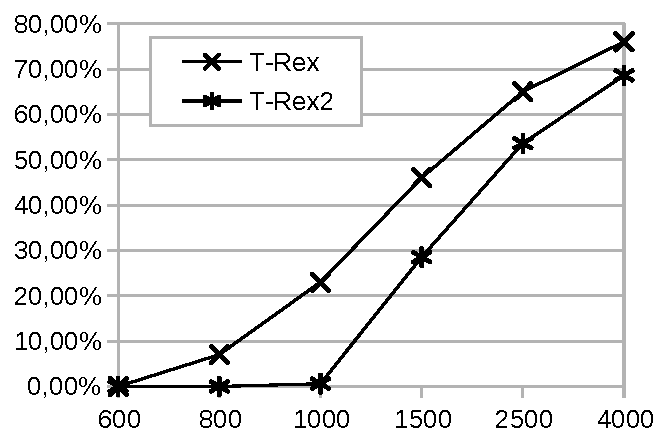
\includegraphics[width=.95\linewidth]{trex_vs_rewrite_freq_drop}
  \caption{TRex vs Rewrite\\
  	Frequencies and drop}
  \label{fig:trex_vs_rewrite_freq_drop}
\end{minipage}%
\begin{minipage}{.5\textwidth}
  \centering
  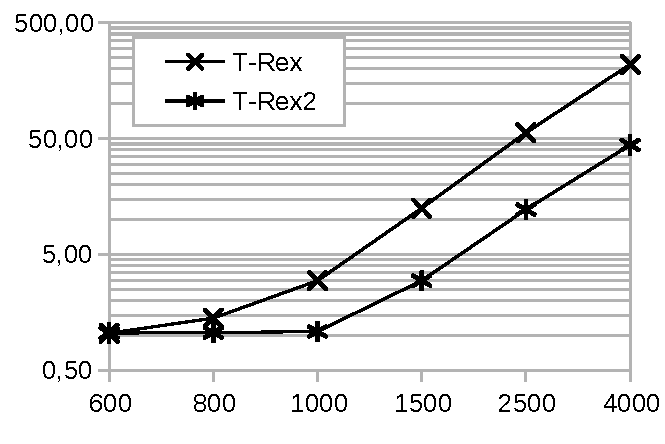
\includegraphics[width=.95\linewidth]{trex_vs_rewrite_freq_time}
  \caption{TRex vs Rewrite\\
  	Frequencies and time}
  \label{fig:trex_vs_rewrite_freq_time}
\end{minipage}
\end{figure}

To better explore the domain we also picked a middle frequency, 1500, and varied the windows size, in a range from 3 to 12.\\
The results, shown in figure \ref{fig:trex_vs_rewrite_win_drop} and \ref{fig:trex_vs_rewrite_win_time}, are directly related to the first measurement and confirm the performance gain.\\
We can also observe how in both the test case the drop rate and the corresponding execution time are closely correlated and most of the time it is possible to switch from one to the other without loosing the qualitative interpretation.
% TODO maybe add the observation that
% they correlate exponentially: that is likely to happen since the system, discarding packages, reduces event retention and a 10\% global reduction, translates in a 10\% at each step of the pattern composition
\begin{figure}[h]
\captionsetup{justification=centering}
\begin{minipage}{.5\textwidth}
  \centering
  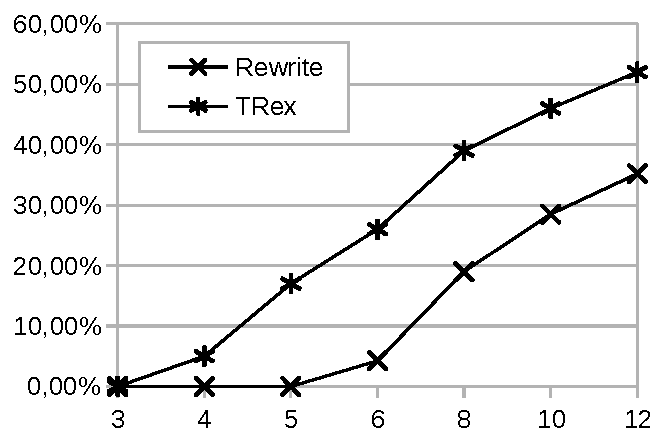
\includegraphics[width=.95\linewidth]{trex_vs_rewrite_win_drop}
  \caption{TRex vs Rewrite\\
  	Windows and drop}
  \label{fig:trex_vs_rewrite_win_drop}
\end{minipage}%
\begin{minipage}{.5\textwidth}
  \centering
  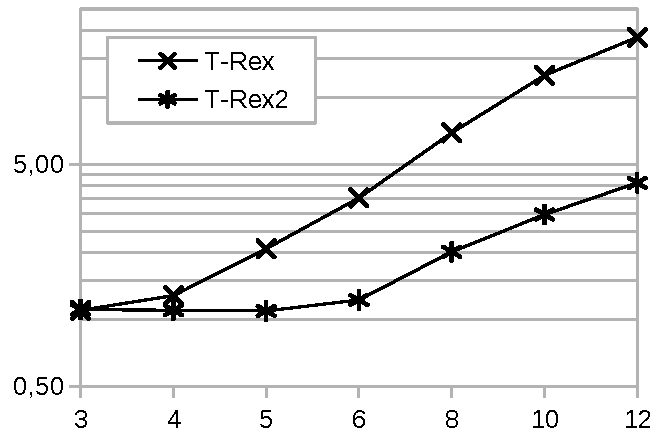
\includegraphics[width=.95\linewidth]{trex_vs_rewrite_win_time}
  \caption{TRex vs Rewrite\\
  	Windows and time}
  \label{fig:trex_vs_rewrite_win_time}
\end{minipage}
\end{figure}

The results were interesting and such an improvement was unexpected, considering that the rewrite closely followed the architecture of its predecessor. The most likely and relevant motivation is a slightly improved parallelism that take advantage of the available processing units, they both had 8 workers threads (plus few other to deal with coordination and event publishing), but the old implementation distribute the jobs statically using rule ids, while the rewrite allocate them dynamically with a thread pool.\\
However it is worth noting that an other good performance improvement was obtained replacing hash-maps with linear-probing ones: in context where the collection contain just few entries, the cost of hashing a value is higher than simply going through the whole vector and this has also a great impact on creation, destruction and clone operations.

\section{Static data}
In this section we are going to introduce the integration between events and persistent data, starting from the simplest configuration and gradually adding variations to validate.\\
This approach reproduce the actual experimentation we followed during the thesis research and it will highlight some phenomena that may look counterintuitive at first glance and natural once understood.

\subsection{Additional variables}
Once again we must refine the domain of the problem, since the new expressivity inevitably causes the expansion of the control variables with the one needed to describe the properties of the database itself and the interaction between the two systems.\\
In particular a database is a complex technology and have plenty of settings and characteristic, but we focused on the fundamental ones: the number of rows, the number of columns, the distribution of the values, the latency of the connection and the presence of indexes.\\
While the integration into the CEP execution is characterized by the selection policy, the constraints on the values, the number of results and the frequency of invocation.

\subsection{Rule adaptation}
The previous TESLA rule was kept as a template and extended with a static predicate with the following configuration:
\begin{align*}
&declare\ SE_0(x:\ int,\ y:\ int)\ with\ id\ 0\\
&declare\ SE_1(x:\ int,\ y:\ int)\ with\ id\ 1\\
&declare\ \ldots\\
&declare\ SE_i(x:\ int,\ y:\ int, z: int)\ with\ id\ i\\
&declare\ SE_{i+1}(col_0:\ int,\ \ldots,\ col_j:\ int)\ with\ id\ i+1\\
&declare\ fact\ SD(col_0:\ int,\ \ldots,\ col_j:\ int)\ with\ id\ i+2\\
&declare\ CE()\ with\ id\ i+3
\end{align*}
\begin{align*}
&from\ SE_0[\$p_0 = y](x == 1)\\
&and\ each\ SE_1[\$p_1 = y](x == 1)\ within\ \tau_1\ from\ SE_0\\
&and\ \ldots\\
&and\ each\ SE_i[\$p_{i,1} = y,\ \$p_{i,2} = z](x == 1)\ within\ \tau_i\ from\ SE_{i-1}\\
&and\ each\ SD[\$c_0 = col_0](col_1 >= \$p_{i,1},\ col_{i,2} < \$p_{i,2})\\
&emit\ CE(x = \$c_0)
\end{align*}
There is a new declaration $SD$ that describe the static data collection and each attribute is mapped to a column of the table. \\
Every simple event now has an additional numerical attribute, which in the rule is always assigned to a parameter: this allow to reference it within the static predicate expanding the variability of the query, which will come in handy when we will evaluate caches. The event $SE_i$ is different, it has a second and third attribute, that are always referenced in the static predicate and combined they work as lower and upper bound, controlling the result of the query.\\
Another declaration was introduced, $SE_{i+1}$, that can be used as a replacement of $SD$ whenever we want to reduce the access to the DB while keeping the same level of produced events.

\subsection{Workload}
% database creation, database random data, extension of the rule (last predicate), 1000 rules 100 declarations, highly frequent and dense, now focused on each sel policy
First of all, to execute the test cases, we needed a valid data-set to work with. The entries generation is characterized by a variable number of rows and a number of columns that we usually kept fixed to two: an incremental index and a numerical payload. The payload was uniformly generated in a range between $-1 / 2 * \#rows$ and $+1 / 2 * \#rows$. The uniform distribution of the data allowed to have a statistically complete population in a non sequential order, to avoid possible bias in term of DBMS architecture or file read.\\
The predicates number per rule is now 4 including the static or substitute predicate and the choice of the last predicate is parameterized with probabilistic threshold. The declaration were changed to 100 groups of 5, plus one single declaration for the database table. The rule defined are 1000, preserving the ratio of 10 identical rule for each declaration group. Database indexing can be switched on or off.\\
The events are still generated uniformly with respect to the declarations. The first attribute is always set to 1, while the second is set randomly according to a selectable probabilistic distribution. Finally the third parameter of $SD_i$ is set to be on average at a given distance (usually 10) from the coupled second parameter, so that they can act properly as lower and upper bounds.

\subsection{Table simulation and database}
The interaction with persisting collections is a need that was already spread, before this and other implementations came to rescue and we already mentioned the workarounds to provide the same functionality without native support. So it seemed appropriate to start the evaluation with a comparison between of the old way and the newly integrated SQLite library.

We had to define two executables with the very same semantic, so we simply applied the algorithm for DB population to produce events with the same payload of the corresponding table and we emitted all of them at the beginning of the execution. At the same time we replaced the static predicate in each rule with one that target the simulated event stream. The new predicate was characterized by an unlimited window, so that the data would be accessible at any time.

\begin{figure}[h]
  \centering
  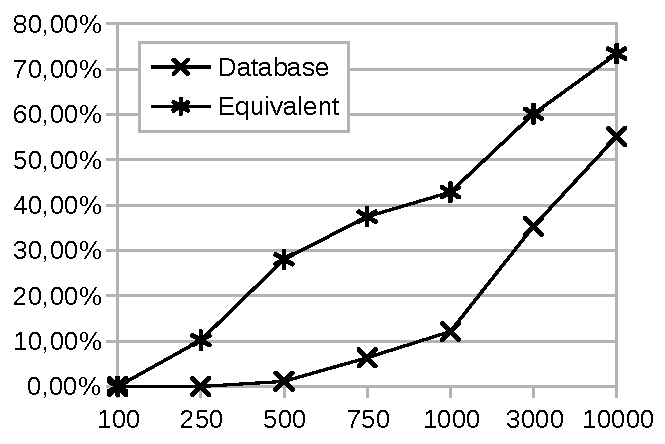
\includegraphics[width=.6\textwidth]{equiv_vs_db_800r_drop}
  \caption{Database vs simulation\\
  Rows and drop}
  \label{fig:equiv_vs_db_800r_drop}
\end{figure}

Once we had both working, we noticed that the performance was poor for both the contenders and we had to constrain ourselves to run the program with a small window of 2s average and low frequency of 800 events per second. However we found that the cardinality of the collection was the most relevant variable in this configuration, so we decided to evaluate that aspect.\\
In figure \ref{fig:equiv_vs_db_800r_drop} we can see the drop rates starting from only 100 elements up to 10000. It's easy to notice how the simulation was perfectly functional only with the minimum settings. The database instead, even without tuning, performed evidently better: managed to handle up to about 500 elements and then kept a noticeable margin over the equivalent.\\
Even if slightly reassuring, the result was far from optimal and we continued the progression toward a reliable setup.

\subsection{Database index}
The turning point was the creation of a table index on the columns frequently queried.\\
In classical DBMS scenarios the use of an index is always a trade off between the cost of keeping it updated and the benefits of a reduced query time. On the opposite side, our system meets exactly the requirements: the data are assumed to be immutable and the queries keep repeating in the same known patterns.\\
Surely we knew it would have a beneficial effect, but the results were beyond any expectation and, even though now it may appear reasonable, at the first impression it was astonishing how changing a simple flag in the DB could drastically change the situation. Every query was satisfied several order of magnitude faster than before and the most valuable fact was that the correlation between speed and number of rows was completely vanished.\\
We tested from 100 to 10 million rows and the time of response is virtually the same, so, after that, the size difference was not considered anymore and the tests were ran with a million of entries. At the same time we observed that preloading the database in memory does not have any benefit over the normal execution and that is probably due to the operating system cache that does it already.

\begin{figure}[h]
  \centering
  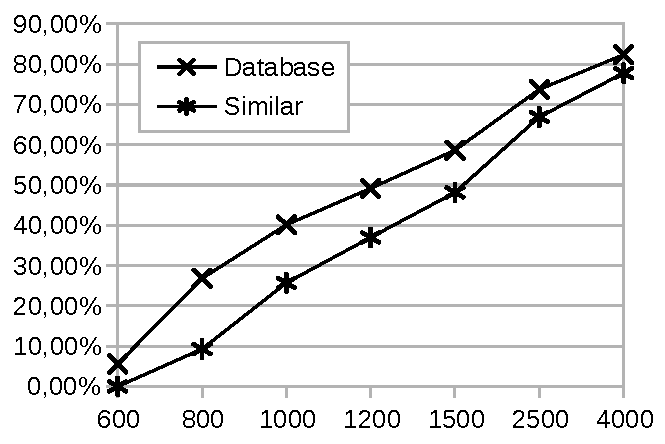
\includegraphics[width=.6\textwidth]{db_or_not_db_drop}
  \caption{Database vs similar load\\
  	Frequency and Drop}
  \label{fig:db_or_not_db_drop}
\end{figure}

To validate the new configuration we made a comparison with an execution that had no static predicates, but would process and generate a similar volume of events. To do so we replaced each predicate of type $SD$ with one of type $SE_{i+1}$, with no constraints and let the window unlimited. Then we generated events of type $SE_{i+1}$ in the same number as the average length of the database result set. In this way the behavior of the system is closely emulated.\\
Since both the setups perform well, to stress the engine we widened the window to 6 seconds on average and analyzed the effects of different frequencies. The results in figure \ref{fig:db_or_not_db_drop} shows how the database access is still behind the classical execution, losing between $10\%$ and $20\%$ more packages. At the same time we can notice how similarly they react to the variation of frequency, meaning that they are in the same league of comparison and there is hope that further optimization would bring reasonable improvements. 

\section{Cache}
The behavior of a CEP engine is often repetitive or predictable with a certain degree of accuracy. For example, it is likely that a train, that sent an event of delay, will signal an additional delay in the near future or that the temperature of a room will oscillate between the same few values. So if we kept track of the previously extracted information we could save some computation.\\
This brings us to the last step of our optimization: the introduction of a cache layer between the CEP engine and the database.

The cache acts transparently to the system so, this time there is no need of adapt declarations and rules.\\
However yet new control variables have to be taken into account. First of all there is the choice of the algorithm among the many presented in the literature, then there is the size in terms of memory occupation and finally there is the possibility to share the storage or split it among the different users. Moreover there are environmental factors that influence the results like the domain and the probabilistic distribution of the values. Finally miss rate and hit and miss time are the characteristic metrics of performance of a cache.

\begin{figure}[h]
  \centering
  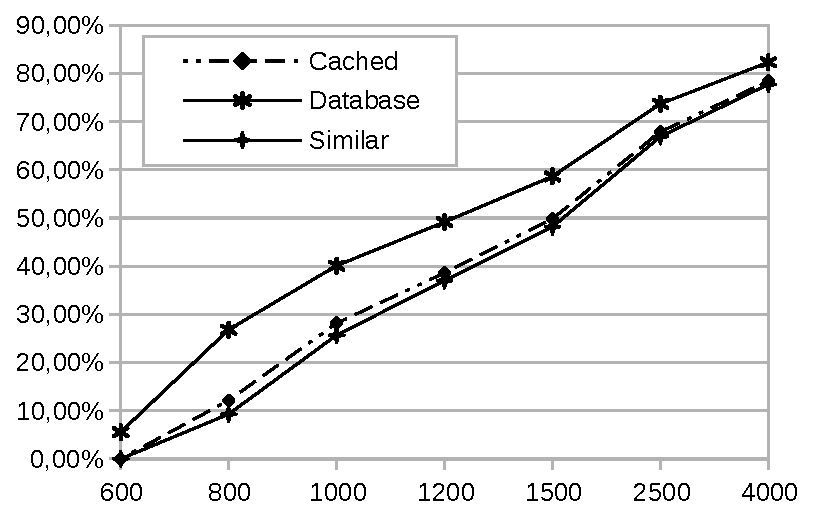
\includegraphics[width=.75\textwidth]{db_or_not_db_cached_drop}
  \caption{Perfect cache - Frequency and Drop}
  \label{fig:db_or_not_db_cached_drop}
\end{figure}

In the figure \ref{fig:db_or_not_db_cached_drop} we can see the previous chart \ref{fig:db_or_not_db_drop} enriched with the result of a cached execution under favorable conditions. Even though it is just a potential optimum, it tease us to finally close the performance gap, that is now barely visible.

\subsection{Shared or per predicate}
When the cache is allocated as a single storage accessed by different predicates, if they request similar data they will share the space and the cache loading cost. Also if there is some process that has more benefits from caching, an advanced algorithm could reward it with more space in memory. However there is always the risk that a single component would hog the entire space, filling it with garbage and degrading the system wide performance.\\
A cache per predicate, instead, would be much smaller, but it could better adapt to the specific pattern or distribution of the data.\\
However we found out to be another the most relevant factor to prefer one model to the other: sharing the cache across multiple threads require constant synchronization. In the implementation the cache is wrapped with a mutex that soon became the bottleneck of the entire parallelization.

\subsection{Data distribution}
First of all we need to clarify that having a discrete and not too dense values domain is a fundamental requirement, otherwise even in the smallest range there would be to many elements to hope for a reasonable match in the cache. So for example floating point numbers usually do not take part to the cache key.\\
The effectiveness of a cache is based on assumptions on the processed data, for example time locality, meaning that a value requested recently is likely to be requested again. Each assumption may fit better or worse depending from the actual data distribution.

The system was built to offer a choice about the distribution of the input event values. So it is possible to experimented with gaussian, exponential and uniform distributions tuning the parameters to spread or narrow the range of the samples.\\
However we found out that this is only partially relevant, in fact there is a limit to the variability that can be introduced by a single event: because of the nature of the system, only a restricted number of events is queued in a processor and that is the maximum expression of the distribution. Conversely sequences of evaluation are executed repeatedly and the same data is requested many time during a single system iteration, so the benefit of the cache prevail over any possible distribution.\\
The situation changes when we make the static predicate dependent from more than one event at a time: in this case the probability distribution combine with each other and generate a wider and more diverse output, challenging the capacity of the cache.

\subsection{Algorithm comparison}
% LRU_SIZE vs GDFS vs COLLISION (not a big difference, why?)
In the previous chapter we explained which cache algorithms were implemented and how each of them works. Now we will analyze the tests of all of them to verify how they fit in the application.

The basic execution configuration we set 2000 event per second and 2 seconds window, with the event payload sampled from a normal distribution $\mathcal{N}(\mu = 0,\ \sigma = 30)$ and with the static query dependent from the last two predicate (expanding the query parameterization space, making harder to cache enough values). Then we varied the cache size, meant as the number of the rows contained in each node, from 500 to 6000.\\
We first analyzed the miss rate of each algorithm, see figure \ref{fig:cache_showdown_miss}, and then compared it to the corresponding drop rate to evaluate the impact on the global execution, see figure \ref{fig:cache_showdown_drop}.

\begin{figure}[h]
  \centering
  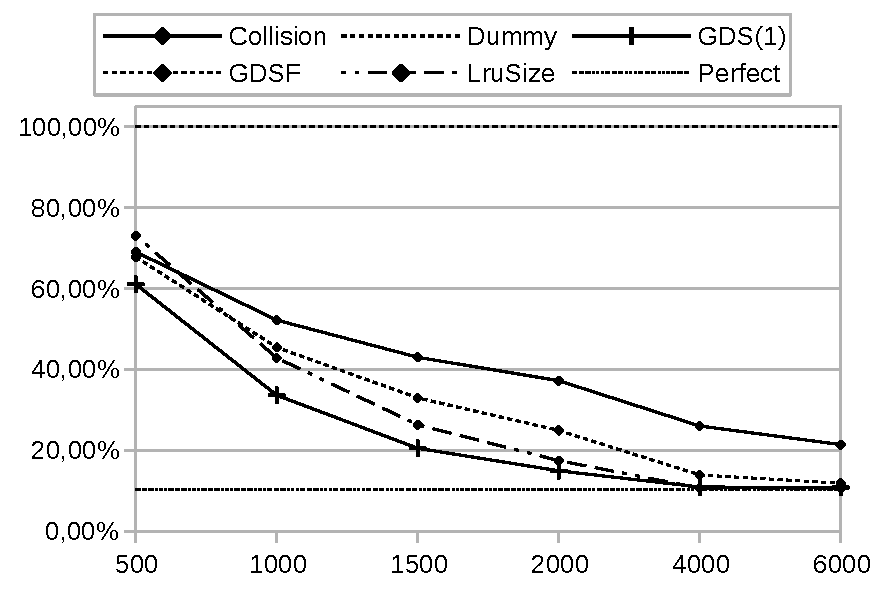
\includegraphics[width=.8\textwidth]{cache_showdown_miss}
  \caption{Cache comparison - Frequency and Miss}
  \label{fig:cache_showdown_miss}
\end{figure}
\begin{figure}[h]
  \centering
  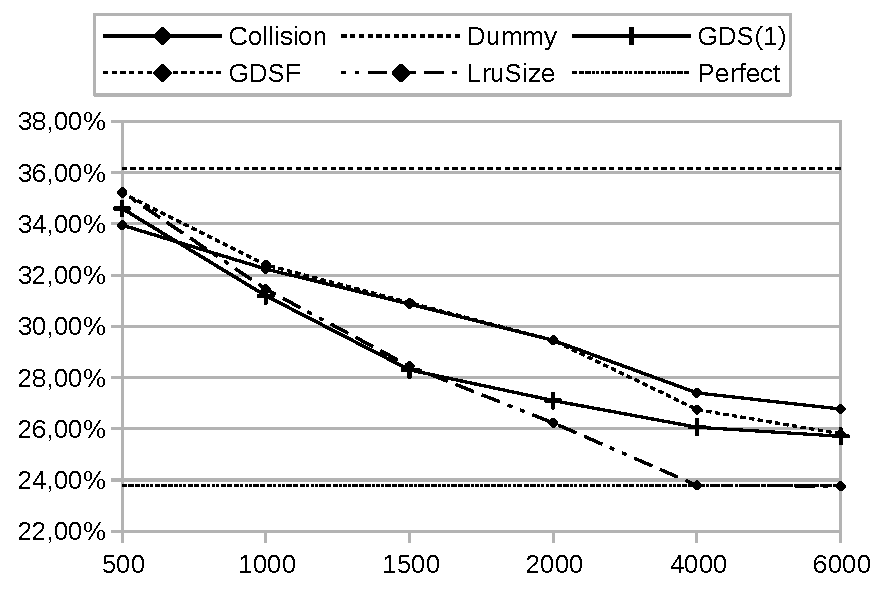
\includegraphics[width=.8\textwidth]{cache_showdown_drop}
  \caption{Cache comparison - Frequency and Drop}
  \label{fig:cache_showdown_drop}
\end{figure}

The dummy cache was used as the example of worst case performances with $100\%$ miss rate. While the perfect cache was used to set the upper limit for the maximum efficiency achievable, with a $10\%$ of miss rate. They are shown on the charts as a horizontal line respectively at the top and at the bottom of the plots. The perfect cache allowed also to estimate to about 12000 the size of the cache necessary to store every received value.\\
The collision cache, that is built on a very basic replacement policy, had a poor performance and was exceeded by every other algorithm. However it was unexpected to see the GDSF cache, that is the de facto standard and champion in HTTP caching, to be clearly left behind in the comparison. My intuition is that its measure of frequency did not work well with the repeated access patterns of a CEP engine.\\
The second best is the LRU (size), that as always, proved itself to be a good allround solution and the first choice for any caching purpose. The winner of the comparison is the GDS(1) cache, that choosing smaller entries is able to maximize the memory usage. We can also notice, that both the top two algorithms reach the level of optimality of the perfect cache with a size between 2000 and 4000 entries, that mean 3 to 6 time less than the actual requirement.

If we compare the results with the plot of system wide performances, we notice that there are some differences and the sole minimization of the miss rate it is not sufficient affect the global execution. The most notable example is how GDS(1), champion of the previous category, fails to keep up with LRU. The phenomenon is explained by the difference in term of hit time: in fact GDS(1) does have more hits (between $5\%$ and $10\%$ more), but pays them almost the double of the LRU ($\sim 1200 \nu s$ compared to $\sim 650 \nu s$ of access time). The reason behind this slow down is likely due to the suboptimal GDS(1) implementation, that I built making use of combination of collection from standard library, instead of crafting and optimize it by hand.

\section{Additional factors}
\subsection{Event selection policy}
% EACH vs FIRST/LAST
\subsection{Percentage of static predicates}
% PERCENTAGE OF STATIC PREDICATES and SATURATION FREQUENCY
\subsection{Parallelism}
% N OF CORES
